\documentclass[11pt
,aspectratio=169
%,draft
]{beamer}
%\usetheme{}
\usepackage[utf8]{inputenc}
\usepackage[german]{babel}
\usepackage[T1]{fontenc}
\usepackage{amsmath}
\usepackage{amsfonts}
\usepackage{amssymb}
%\usepackage[citestyle=authoryear,bibstyle=authoryear,backend=biber]{biblatex}
\usepackage[justification=raggedleft, font=tiny, labelfont={color=mba-col-fg2,bf}, tableposition=bottom, format=hang]{caption}
\usepackage{csquotes}
\usepackage{graphicx}
\usepackage{xcolor}

\usepackage{hyperref}
%\usepackage[hyphenbreaks]{breakurl}

\author{Ahmed, Amir, Matthias, Omar und Salim}
\title{Pocket Monster}
\subtitle{in JavaFX}
%\setbeamercovered{transparent} 
\setbeamertemplate{navigation symbols}{} 
\setbeamertemplate{caption}[numbered]
\logo{
\includegraphics[width=25ex]{luh_logo.eps}} 
\institute{Programmieren II an der Leibniz Universität Hannover} 
\date{14.~Juli~2025} 
\subject{(Quanten-)Physik} 


\hypersetup{
    pdftitle = {Präsentation - Implementation von Pocket Monster},
    pdfauthor = {Ahmed Amine Kortas, Amir Abid, Matthias-Benjamin Ahrens, Omar Ennabli und Salim Nahdi},
    pdfsubject = {Bericht über die implementieren von Pocket Monsters in JavaFX im Rahmen der Gruppenaufgabe in Programmieren II},
    pdfkeywords = {Programmieren, JavaFX, Leibniz Universität Hannover, Gruppenaufgabe, Pocket Monsters},
colorlinks=true,
linkcolor=mba-col-link,
citecolor=mba-col-link,
filecolor=mba-col-link,
urlcolor=mba-col-link,
naturalnames
}


\definecolor{mba-col-uni}{HTML}{1E5D99}
\definecolor{mba-col-link}{HTML}{008080}
\definecolor{mba-col-bg}{HTML}{272727}
\definecolor{mba-col-fg}{HTML}{ffffff}
\definecolor{mba-col-fg2}{HTML}{999999}


\setbeamercolor{background canvas}{bg=mba-col-bg}
\setbeamercolor{normal text}{fg=mba-col-fg}
\setbeamercolor{frametitle}{fg=mba-col-uni}
\setbeamercolor{title}{fg=mba-col-uni}
\setbeamercolor{section in toc square}{fg=mba-col-uni-2}
\setbeamercolor{item}{fg=mba-col-uni}

\setlength{\itemsep}{0pt}

\begin{document}

\begin{frame}
\titlepage
\end{frame}

%\begin{frame}{Gliederung}
%\tableofcontents
%\end{frame}

\begin{frame}
\begin{center}
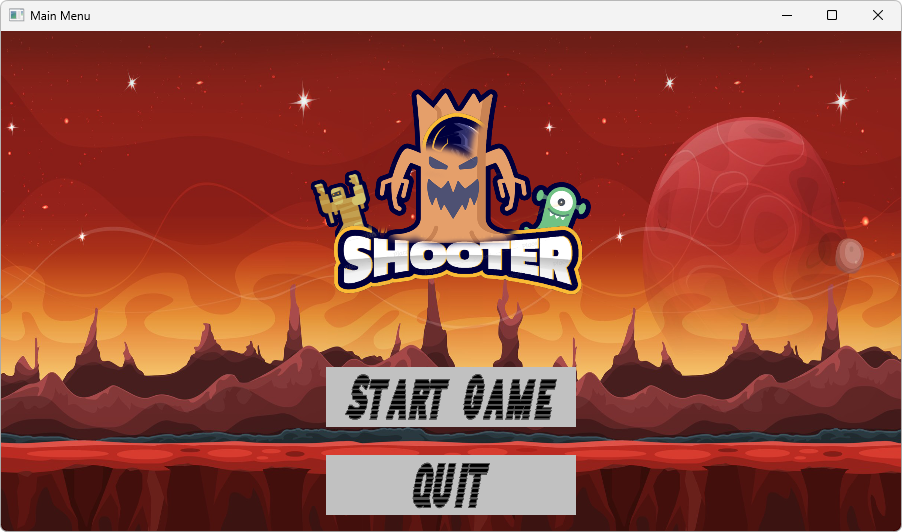
\includegraphics[scale=.5]{img/MainMenu.png}
\end{center}
\end{frame}

\begin{frame}
\begin{center}
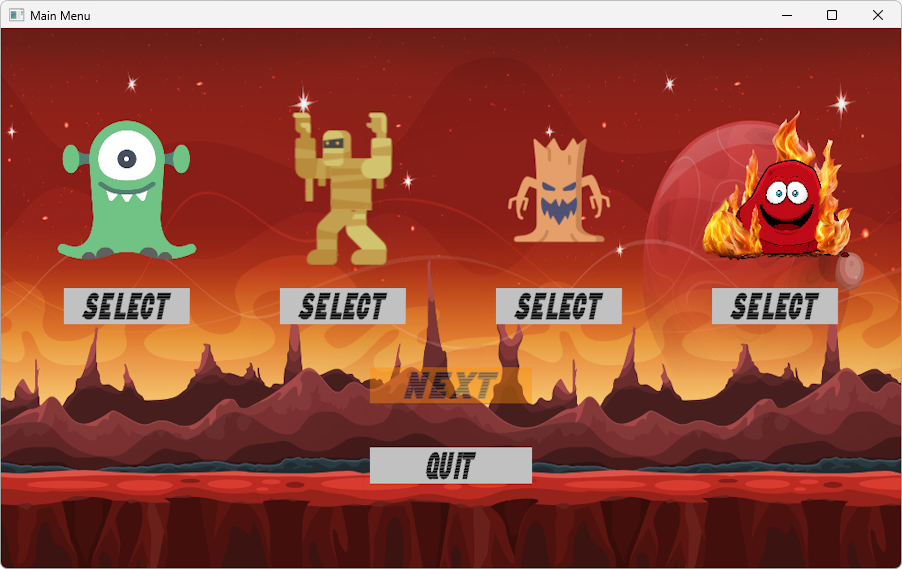
\includegraphics[scale=.5]{img/Selector.png}
\end{center}
\end{frame}

\begin{frame}{Alien}
\begin{minipage}{.3\linewidth}

\includegraphics[width=\linewidth]{img/Alien.png}
\end{minipage}\hfill
\begin{minipage}{.65\linewidth}
\begin{description}
\item[Element] Wasser
\item[Attacks] Slimy Punch (15hp), UFO Blast (30hp)
\item[Max HP] 200
\end{description}
\end{minipage}
\end{frame}

\begin{frame}{Tree Monster}
\begin{minipage}{.65\linewidth}
\begin{description}
\item[Element] Grass
\item[Attacks] Root Whip (18hp), Earthquake (40hp)
\item[Max HP] 210
\end{description}
\end{minipage}\hfill
\begin{minipage}{.3\linewidth}

\includegraphics[width=\linewidth]{img/Tree.png}
\end{minipage}
\end{frame}

\begin{frame}{Mummy}
\begin{minipage}{.3\linewidth}

\includegraphics[width=\linewidth]{img/Mummy.png}
\end{minipage}\hfill
\begin{minipage}{.65\linewidth}
\begin{description}
\item[Element] Rock
\item[Attacks] Wrap Attack (10hp), Ancient Curse (35hp)
\item[Max HP] 200
\end{description}
\end{minipage}
\end{frame}

\begin{frame}{Rock Golem}
\begin{minipage}{.65\linewidth}
\begin{description}
\item[Element] Fire
\item[Attacks] Stone Fist (20hp), Meteor Slam (45hp)
\item[Max HP] 220
\end{description}
\end{minipage}\hfill
\begin{minipage}{.3\linewidth}

\includegraphics[width=\linewidth]{img/Rock.png}
\end{minipage}
\end{frame}



\begin{frame}
\begin{center}
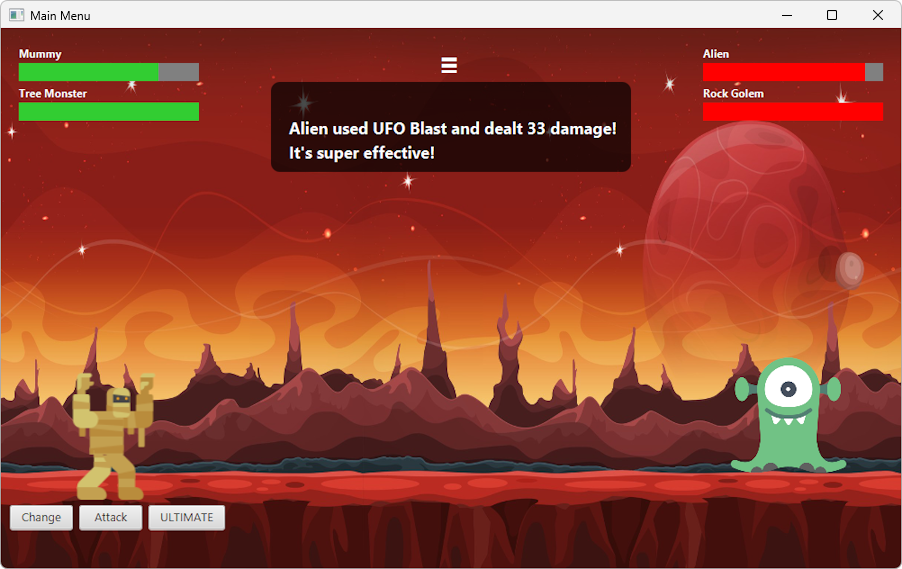
\includegraphics[scale=.5]{img/Game.png}
\end{center}
\end{frame}


\begin{frame}
\begin{center}
\textbf{{\Huge Live Demo}}
\end{center}
\end{frame}

\end{document}